% !TEX TS-program = pdflatex
% !TEX encoding = UTF-8 Unicode

% This is a simple template for a LaTeX document using the "article" class.
% See "book", "report", "letter" for other types of document.

\documentclass[11pt]{article} % use larger type; default would be 10pt

\usepackage[utf8]{inputenc} % set input encoding (not needed with XeLaTeX)

%%% Examples of Article customizations
% These packages are optional, depending whether you want the features they provide.
% See the LaTeX Companion or other references for full information.

%%% PAGE DIMENSIONS
\usepackage{geometry} % to change the page dimensions
\geometry{a4paper} % or letterpaper (US) or a5paper or....
% \geometry{margin=2in} % for example, change the margins to 2 inches all round
% \geometry{landscape} % set up the page for landscape
%   read geometry.pdf for detailed page layout information

\usepackage{graphicx} % support the \includegraphics command and options
\graphicspath{ {./images/} }

% \usepackage[parfill]{parskip} % Activate to begin paragraphs with an empty line rather than an indent

%%% PACKAGES
\usepackage{booktabs} % for much better looking tables
\usepackage{array} % for better arrays (eg matrices) in maths
\usepackage{paralist} % very flexible & customisable lists (eg. enumerate/itemize, etc.)
\usepackage{verbatim} % adds environment for commenting out blocks of text & for better verbatim
\usepackage{subfig} % make it possible to include more than one captioned figure/table in a single float
% These packages are all incorporated in the memoir class to one degree or another...

%%% HEADERS & FOOTERS
\usepackage{fancyhdr} % This should be set AFTER setting up the page geometry
\pagestyle{fancy} % options: empty , plain , fancy
\renewcommand{\headrulewidth}{0pt} % customise the layout...
\lhead{}\chead{}\rhead{}
\lfoot{}\cfoot{\thepage}\rfoot{}

%%% SECTION TITLE APPEARANCE
\usepackage{sectsty}
\allsectionsfont{\sffamily\mdseries\upshape} % (See the fntguide.pdf for font help)
% (This matches ConTeXt defaults)

%%% ToC (table of contents) APPEARANCE
\usepackage[nottoc,notlof,notlot]{tocbibind} % Put the bibliography in the ToC
\usepackage[titles,subfigure]{tocloft} % Alter the style of the Table of Contents
\renewcommand{\cftsecfont}{\rmfamily\mdseries\upshape}
\renewcommand{\cftsecpagefont}{\rmfamily\mdseries\upshape} % No bold!

%%% END Article customizations

%%% The "real" document content comes below...

\title{COMP 6320 Design and Analysis of Computer Networks: Course Project}
\author{James S. L. Browning and Austin David Preston}
%\date{} % Activate to display a given date or no date (if empty),
         % otherwise the current date is printed 

\begin{document}
\maketitle

\section{Introduction}

The purpose of this project was to develop a basic simulation of a queueing system. The system simulates two queues, each with its own server for “processing” simulated packets. The system either assigns new arrivals to a queue randomly, or assigns them to the whichever queue is shortest (randomly if they happen to be the same length when a new packet arrives). In addition to a choice of queue assignment strategy, the simulator takes two integer parameters, $\lambda$ and $\mu$, representing the average time between arrivals and the average time needed to service a packet, respectively. Our simulator uses these values to generate appropriate interarrival and service times for the simulator, which uses a while loop and several timer variables to simulate the system millisecond-by-millisecond.

\section{Usage}

The simulator can be compiled using the following command:

\begin{center}
\texttt{gcc main.c -lm -o main}
\end{center}

The first parameter passed to it during usage should be either a \texttt{1} or a \texttt{2}, to select random assignment or minimum queue length assignment, respectively. This should be followed by $\lambda$ and $\mu$ values. For example, this would be a valid usage:

\begin{center}
\texttt{./main 1 10 10}
\end{center}

\section{Performance Data}

\subsection{Lambda}

The figure below shows the change in blocking probability relative to $\lambda$, assuming a constant average service time (here 10 milliseconds). $\lambda$ values were shifted from 1 to 25. At around a $\lambda$ of 5, the service time began to catch up to the growing interarrival time, and beyond a $\lambda$ of 10, the blocking probability reached zero (meaning all arrivals were able to be processed — this was somewhat expected, as at this point, the interarrival time had exceeded the average service time).

\begin{center}
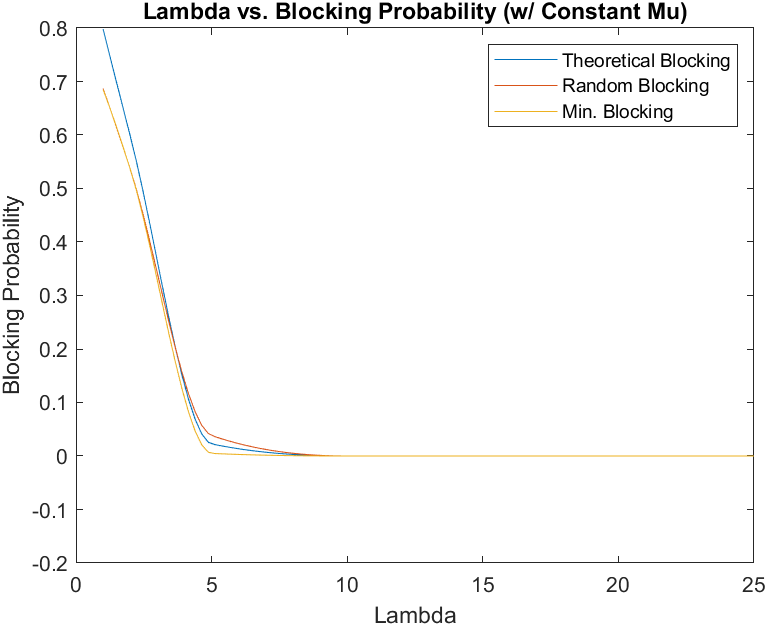
\includegraphics[width=.875\textwidth]{1}
\end{center}

This data demonstrated that $\lambda$ has a significant impact on system performance, though is only relevant to the extent that it outpaces the service time.

The second figure below shows the change in average queue length (over a run of 10,000 packets) relative to $\lambda$.

\begin{center}
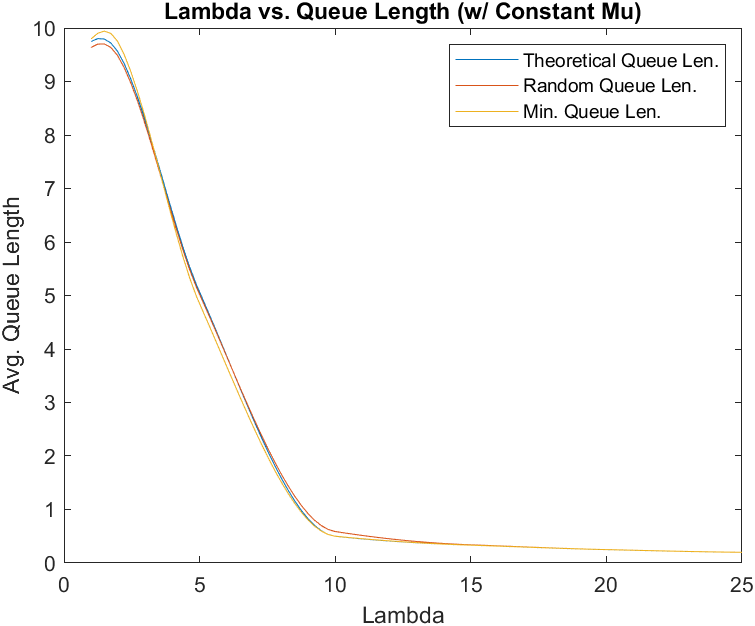
\includegraphics[width=.875\textwidth]{2}
\end{center}

This value shifts downward more gradually, with rapid arrivals quickly filling up the queues, and slower paces allowing them to stay comparatively short. The split queues could be a contributing factor to changes in $\lambda$ having less extreme impacts on queue length than blocking probability, as seen in the first figure.

Finally, the third figure below shows $\lambda$ vs. average sojourn time.

\begin{center}
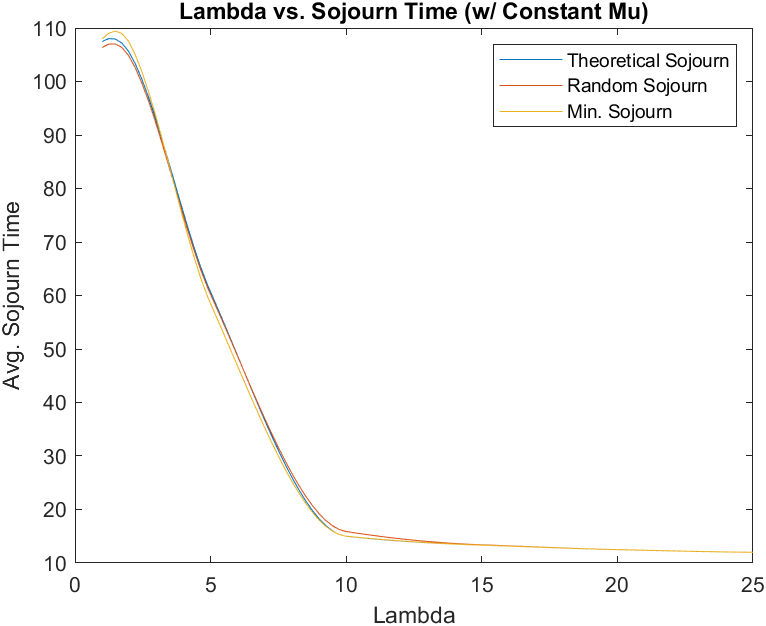
\includegraphics[width=.875\textwidth]{3}
\end{center}

This figure is quite similar to the second figure, showing $\lambda$ vs. queue length, which makes sense — queue length directly correlates with sojourn time, as the number of packets waiting in front of a given packet determines how long that packet will have to wait to be serviced.

\subsection{Mu}

The next figure shows average service time vs. blocking probability.

\begin{center}
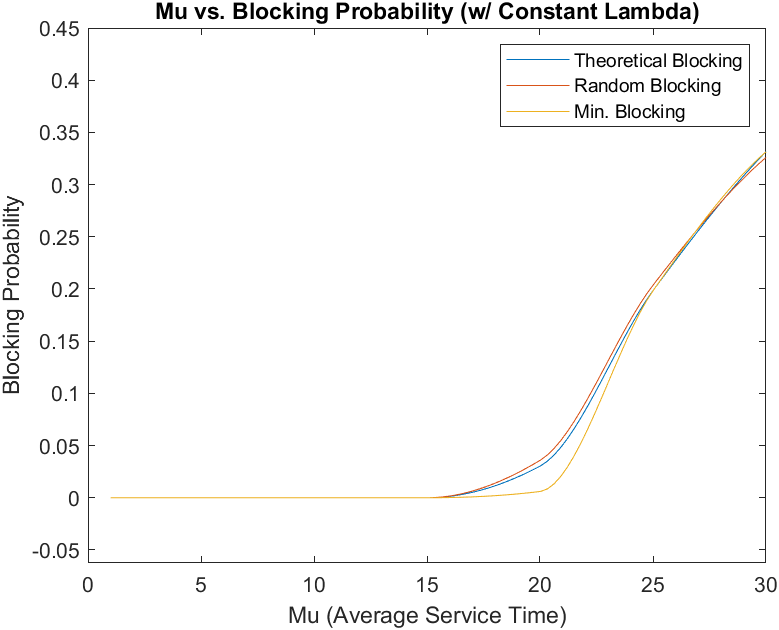
\includegraphics[width=.875\textwidth]{4}
\end{center}

This figure is essentially an inverse of $\lambda$ vs. blocking probability, as increasing the amount of time needed for a packet to be serviced would necessarily increase the odds that some packets would be left behind entirely. The blocking probability does appear to climb more gradually here than it shrank in the first figure, however, perhaps indicating that $\lambda$ carries more weight for this performance metric.

The fifth figure below shows average service time vs. average queue length.

\begin{center}
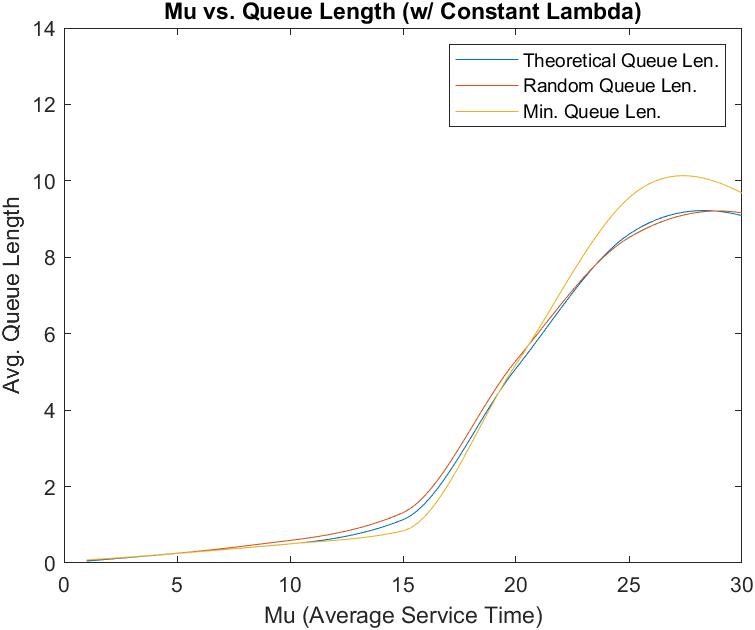
\includegraphics[width=.875\textwidth]{5}
\end{center}

As one might expect, slowing down service time leads to an increase in average queue length. It is interesting to note that the minimum queue length assignment strategy displays a noticeable bump in average queue length at slow service rate values — this is likely because the minimum queue length strategy ensures both queues are being filled equally (meaning they both end up being fully taken advantage of), slightly increasing the average queue length.

The sixth figure below shows average service time vs. average sojourn time.

\begin{center}
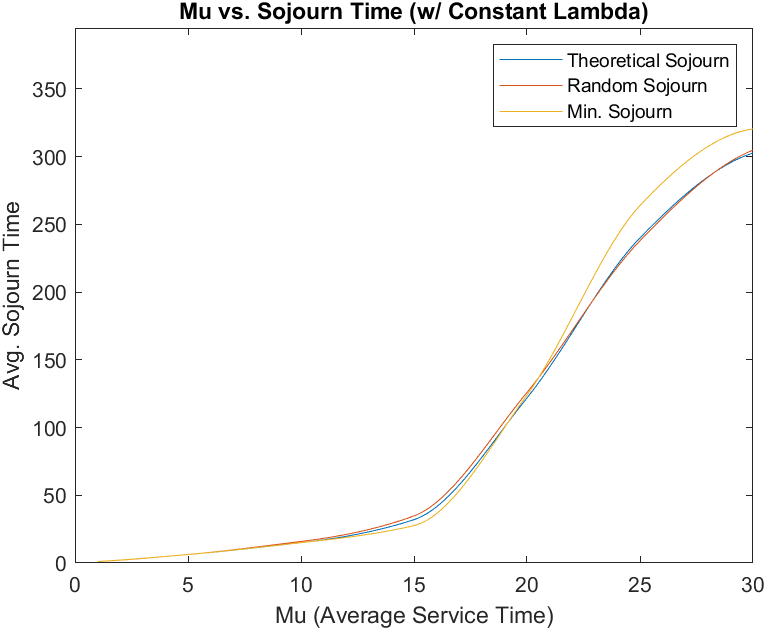
\includegraphics[width=.875\textwidth]{6}
\end{center}

Once again, the outcome here is what one would expect — slowing down service increases sojourn time. As with the figures in the subsection above, this one displays a similarity to service time vs. blocking probability, as the longer a packet is likely to wait for service, the more likely a subsequent packet is to be to dropped entirely.

\subsection{Load}

These next three figures show the above performance metrics relative to the overall load on the system, equal to $\frac{\lambda}{2 \mu}$.

The first figure shows load vs. blocking probability.

\begin{center}
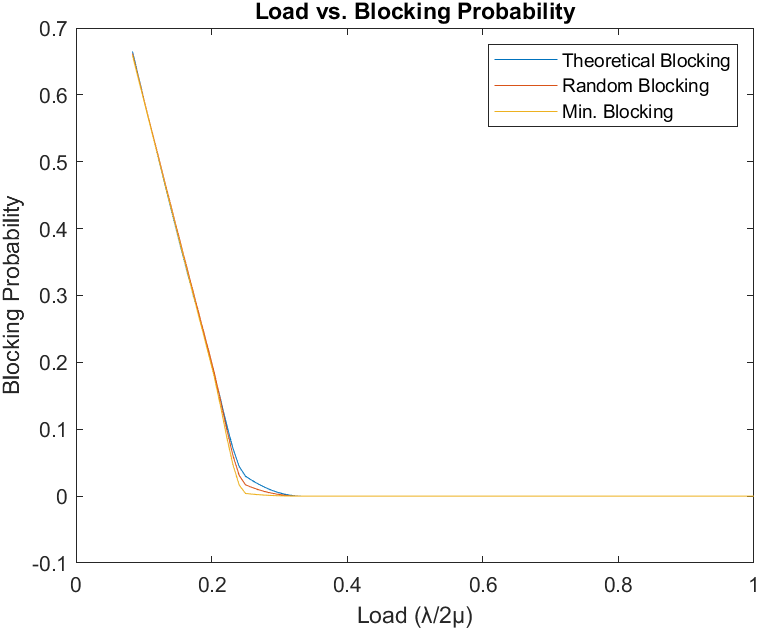
\includegraphics[width=.875\textwidth]{7}
\end{center}

The data above shows that the blocking probability of the system decreases as the average service time speeds up and the interarrival time for packets slows down. The system performs at its best when arrivals are few and far between, and when the servers are able to service those packets quickly.

\begin{center}
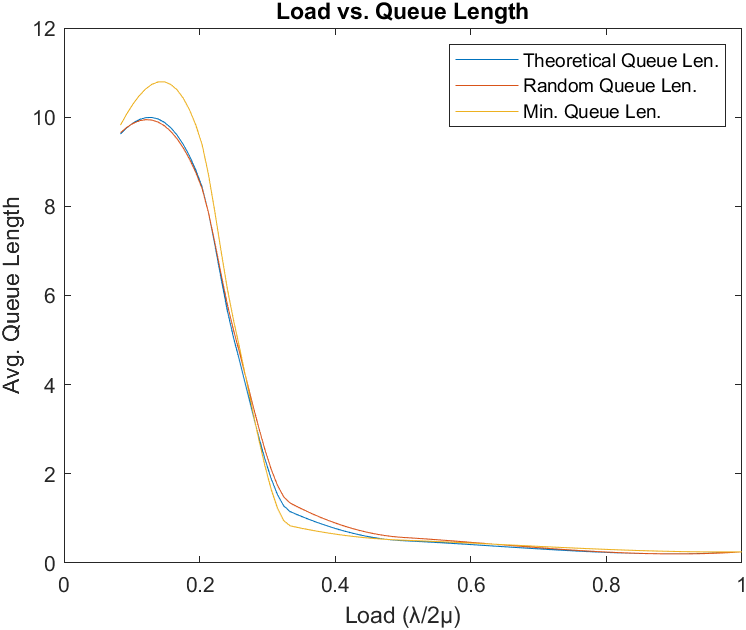
\includegraphics[width=.875\textwidth]{8}
\end{center}

The figure above paints a similar picture — as arrivals become more common and servicing takes longer, the average queue length grows, as more and more packets get backed up in the system.

\begin{center}
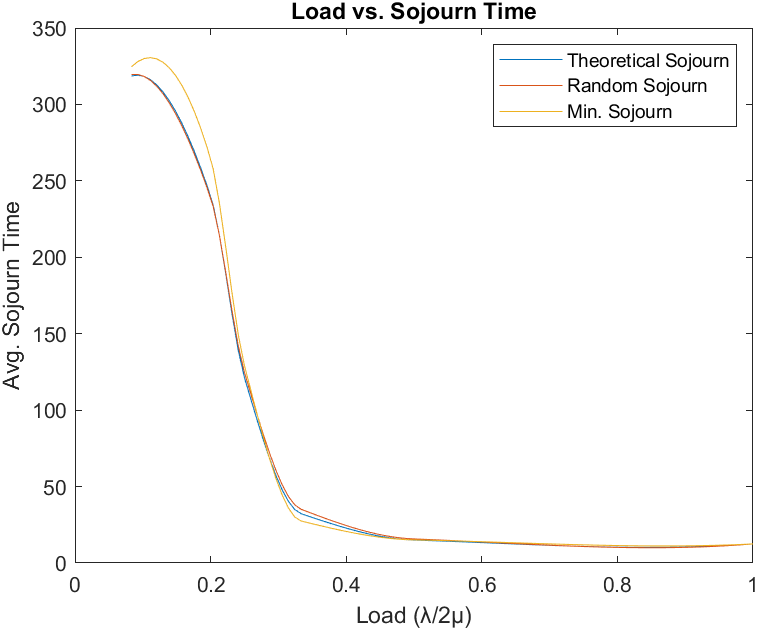
\includegraphics[width=.875\textwidth]{9}
\end{center}

The third and final figure above is quite similar to the previous figure. As queue length decreases, so too does sojourn time, as packets have fewer packets waiting in front of them.

\section{Final Thoughts}

This experiment showed that interarrival time and service time both have an impact on the performance of a system. Interarrival time has a stronger correlation with average queue length, as can be seen in the second figure in section 3.1. More common arrivals mean more packets get backed up, but as long as the average service time is decent, packets will still be processed fast enough for most of them to make it through the system. It is only at extraordinarily high arrival rates that the blocking probability makes a sharp increase, indicating that overall, the service rate has a more consistent correlation with blocking probability (as can be seen in the first figure of section 3.2).

\end{document}
